\begin{frame}
\begin{block}{\textbf{Question}}
How can we summarize models like this in a manner that enables us to \textbf{derive the associated constraints} automatically from the model description so that we can \textbf{compare alternative models}?
\end{block}
\begin{block}{\textbf{Graphical models}}
For example, for the cover of genotype space given by
$\mathcal{G} = \{\{l_1,l_2 \},\{l_1,l'_2 \},\{l'_1,l_2\},\{l'_1,l'_2\} \}$
there is an associated graph, in this case the 4-cycle (also referred to as C4):
\begin{center}
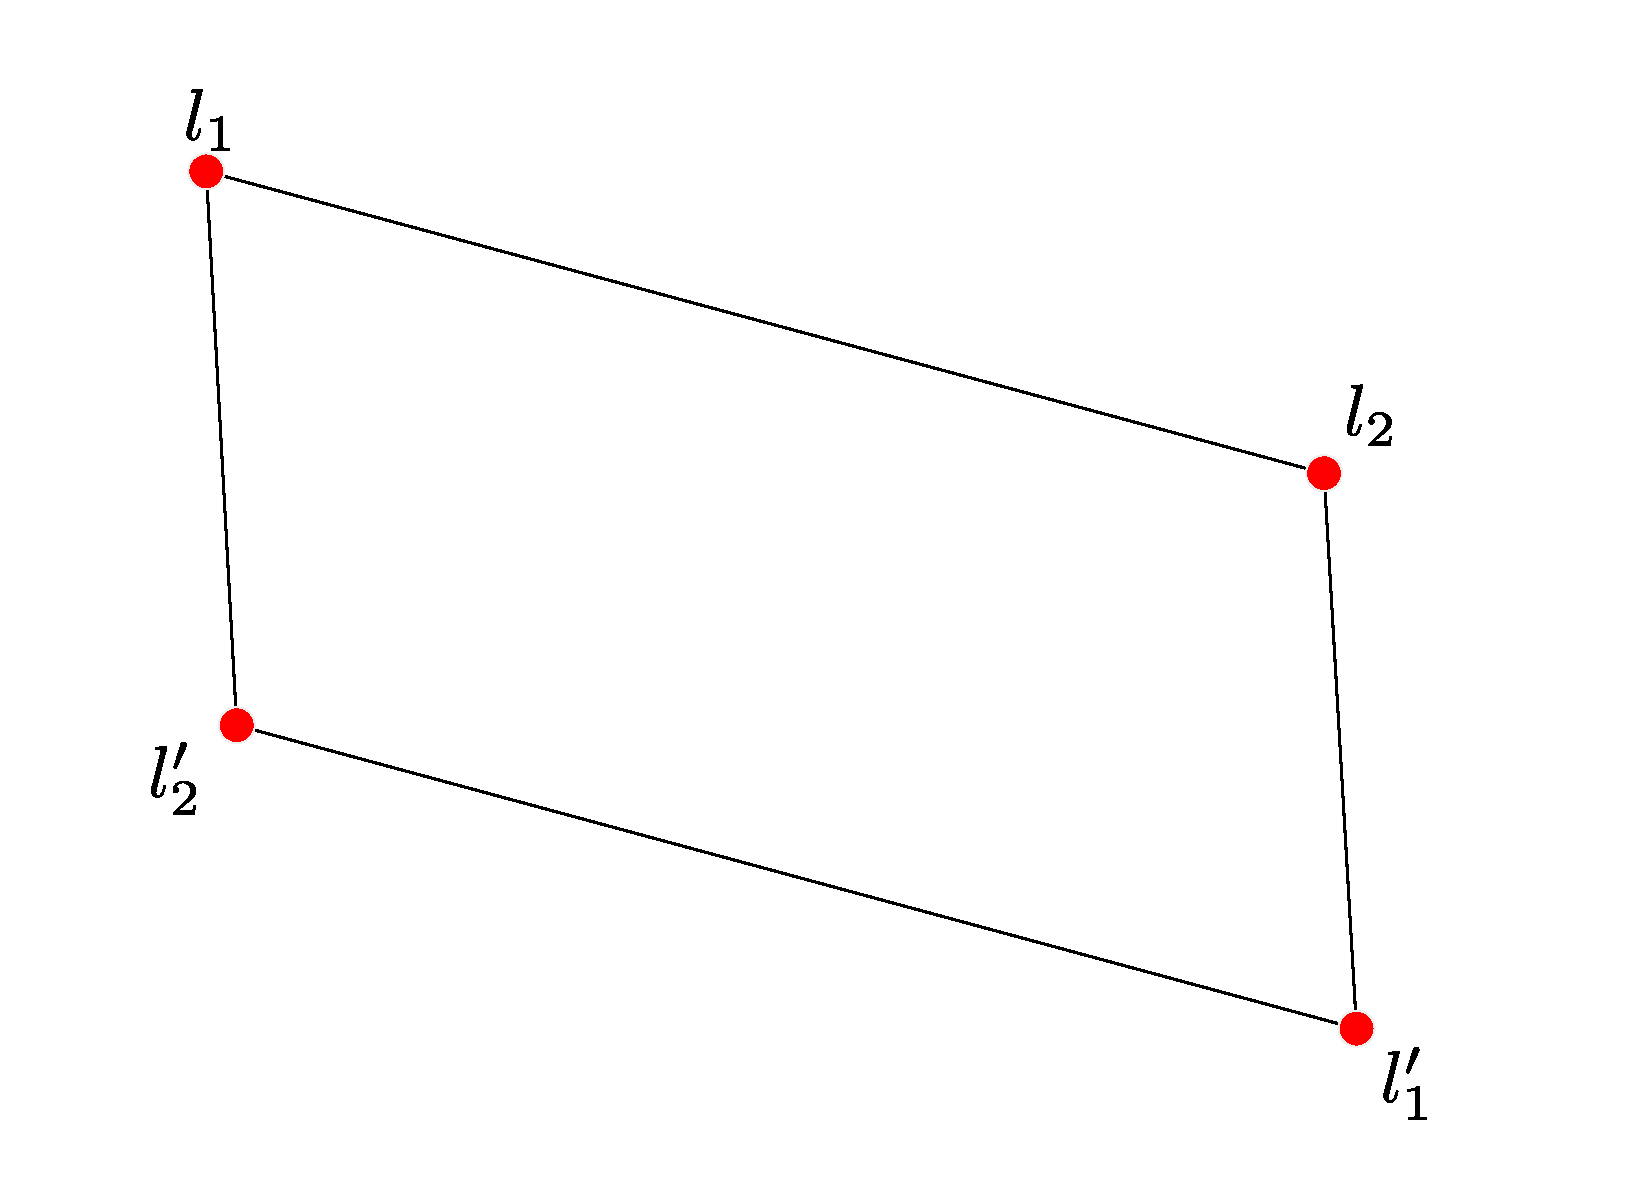
\includegraphics[width=0.4\textwidth]{fig/C4graph_labelled.pdf}
\end{center}
\end{block}
\end{frame}
